\documentclass[11pt,a4paper,oneside]{article}

%%% Работа с русским языком
\usepackage{cmap}					% поиск в PDF
\usepackage{mathtext} 				% русские буквы в фомулах
\usepackage[T2A]{fontenc}			% кодировка
\usepackage[utf8]{inputenc}			% кодировка исходного текста
\usepackage[english,russian]{babel}	% локализация и переносы

\usepackage{blindtext}

\usepackage{fancyhdr}

\usepackage{lipsum}
\usepackage{etoolbox}
\usepackage{color}

%%% Работа с картинками
\usepackage{graphicx}  % Для вставки рисунков
\graphicspath{{data/}}  % папки с картинками
\setlength\fboxsep{3pt} % Отступ рамки \fbox{} от рисунка
\setlength\fboxrule{1pt} % Толщина линий рамки \fbox{}
\usepackage{wrapfig} % Обтекание рисунков и таблиц текстом
\usepackage[export]{adjustbox}
\usepackage{subcaption}
\usepackage{float}

%%% Дополнительная работа с математикой
\usepackage{amsmath,amsfonts,amssymb,amsthm,mathtools} % AMS
\usepackage{icomma} % "Умная" запятая: $0,2$ --- число, $0, 2$ --- перечисление

\title{Контрольная работа по теме \protect\\ "Элементы теории нечетких множеств" \protect\\ Вариант 11}
\date{2020}
\author{Снопов П.М.}


\newenvironment{problem}{
	\medskip
	\begin{problem-internal}
	}{
	\end{problem-internal}
}

\newenvironment{solution}{
	\begin{proof}[Решение]
		\vspace{-8px}
		\setlength{\parskip}{4px}
		\setlength{\parindent}{0px}
	}{
	\end{proof}
}

\newtheorem{problem-internal}{}

\DeclarePairedDelimiter\abs{\lvert}{\rvert}%

\begin{document}
	\maketitle
	\begin{problem}
		Пусть заданы функции принадлежности термов {\bf малая и большая} лингвистической переменной {\bf Величина}
		\begin{equation*}
			\centering
			\begin{aligned}\mu_{мал}(x) = 
			\left\{
			\begin{aligned}
			&1\text{, если $0\leq x \leq 1$,}\\
			&2-x\text{, если $1\leq x \leq 2$,} \\
			&0\text{, если  $x \geq 2$.}
			\end{aligned}
			\right.
			\end{aligned}
			\quad\quad
			\centering
			\begin{aligned}\mu_{сред}(x) = 
			\left\{
			\begin{aligned}
			&0\text{, если $0\leq x \leq 5$,}\\
			&x-5\text{, если $5\leq x \leq 6$,} \\
			&1\text{, если  $x \geq 6$.}
			\end{aligned}
			\right.
			\end{aligned}
		\end{equation*}
		Постройте функцию принадлежности высказывания: {\bf величина $x$ очень мала или величина $x$ более или менее средняя.}(Указание: модификатору {\bf очень} соответствует показатель степени $2$; модификатору {\bf более или менее} соответствует показатель степени $0.5$)
	\end{problem}
	\begin{solution}
		\begin{enumerate}
			\item $ \mu_{очень\; мала}(x) = \mu_{мала}^2(x) \Rightarrow $
			\[
				\mu_{очень\; мала}(x)  = \left\{\begin{aligned}
											 &1\text{, если $0\leq x \leq 1$,}\\
											 &(2-x)^2\text{, если $1\leq x \leq 2$,} \\
											 &0\text{, если  $x \geq 2$.}
										 \end{aligned}\right.
			\]
			\item $ \mu_{более \; менее \; средняя}(x) = \mu_{средняя}^{\frac{1}{2}}(x) \Rightarrow $
			\[
				\mu_{очень\; мала}(x)  = \left\{\begin{aligned}
											&0\text{, если $0\leq x \leq 5$,}\\
											&\sqrt{x-5}\text{, если $5\leq x \leq 6$,} \\
											&1\text{, если  $x \geq 6$.}
										\end{aligned}\right.
			\]
			\item Тогда $ \mu^\ast(x) = \max\{\mu_{очень\; мала}(x),\mu_{очень\; мала}(x)\}  \Rightarrow$
			\[
				\mu^\ast(x) = \left\{ \begin{aligned}
											&1\text{, если $0\leq x \leq 1$\; и $x \geq 6$,}\\
											&(2-x)^2\text{, если $1\leq x \leq 2$,} \\
											&\sqrt{x-5}\text{, если $5\leq x \leq 6$,} \\
											&0\text{, если  $2\leq x \leq 5$.}
				\end{aligned}\right.
			\]
		\end{enumerate}
	\end{solution}
	\begin{problem}
		Обобщенное гауссово число задается функцией принадлежности:
		\[ g(a,\sigma,\beta,x) = e^{-\frac{1}{2}( \frac{x-a}{\sigma})^{2\beta}} \]
		Определите линейный индекс нечеткости и исследуйте его зависимость от параметров.
	\end{problem}
	\begin{solution}
		Попробуем символьно найти решение. Для начала положим $U \coloneqq [-10,10]$. Теперь найдем обычное множество, максимально приближенное к обобщенному гауссову числу $G$:
		\[
			\underline{G} := \{ x \in U: g(a,\sigma,\beta,x) >= 0.5 \}
		\]
		То есть индикаторная функция для $\underline{G}$ имеет вид:
		\[
			1_{\underline{G}}(x) = \left\{\begin{aligned}
												&1\text{, если $g(a,\sigma,\beta,x) >= 0.5$,}\\
												&0\text{, иначе.}
											\end{aligned}
									\right.
		\]
		Найдем множество $\underline{G}$: так как $ g(a,\sigma,\beta,x) >= 0.5$, то:
		\begin{gather*}
			e^{-\frac{1}{2}( \frac{x-a}{\sigma})^{2\beta}} >= 0.5 \\
			-\frac{1}{2} \left( \frac{x-a}{\sigma}\right)^{2\beta} >= -\ln(2) \\
			\left(\frac{x-a}{\sigma}\right)^{2\beta} <= 2\ln(2) \\
			(x-a)^{2\beta} <= \sigma^{2\beta}2\ln(2) \\
			\sum_{k=0}^{2\beta} {2\beta\choose k} x^{2\beta-k}(-a)^k <= \sigma^{2\beta}2\ln(2) \\
			\abs{x-a} <= \sigma({2\ln(2)})^\frac{1}{2\beta}
		\end{gather*}
		Таким образом: \[
		\underline{G} = \{ x \in U : x <= a + \sigma({2\ln(2)})^\frac{1}{2\beta} \; \land\;x >= a - \sigma({2\ln(2)})^\frac{1}{2\beta} \}
		\]
		Тогда линейный индекс нечеткости $\nu$ выглядит следующим образом:
			\[
				\nu(G) = \frac{1}{b-a} \sum_{i=1}^{\infty} \abs{\mu_G(x_i) - 1_{\underline{G}}(x_i)}
			\]
		С помощью {\it Python} исследуем зависимость линейного индекса нечеткости от параметров, положив $U \coloneqq \{-10, ..., 10\} \; : \; \abs{U} = 100$, тогда линейный индекс нечеткости имеет вид:
		\[
		\nu(G) = \frac{1}{100} \sum_{i=1}^{100} \abs{\mu_G(x_i) - 1_{\underline{G}}(x_i)}
		\]
		Тогда имеем:
		\begin{enumerate}
			\item Зависимость обобщенного гауссова числа от параметра $a$ (рис. \ref{fig:a}).
			\begin{figure*}[!hbtp]
				\centering
				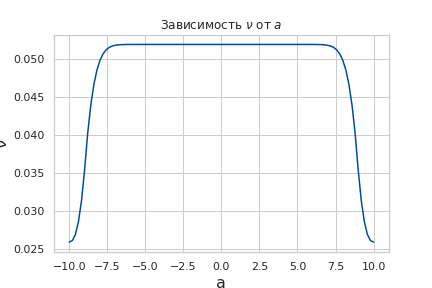
\includegraphics[width=\linewidth]{2ndtaskwitha.png}
				\caption{Зависимость обобщенного гауссова числа от $a$}
				\label{fig:a}
			\end{figure*}
			\item Зависимость обобщенного гауссова числа от параметра $\sigma$ (рис. \ref{fig:sigma}).
			\begin{figure*}[!hbtp]
				\centering
				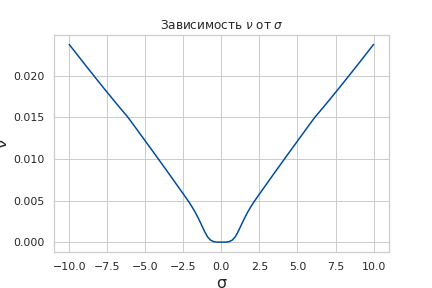
\includegraphics[width=\linewidth]{2ndtaskwithsigma.png}
				\caption{Зависимость обобщенного гауссова числа от $\sigma$}
				\label{fig:sigma}
			\end{figure*}
			\item Зависимость обобщенного гауссова числа от параметра $\beta$(где $\beta \in \mathbb{N}$) (рис. \ref{fig:beta}).
			\begin{figure*}[!hbtp]
				\centering
				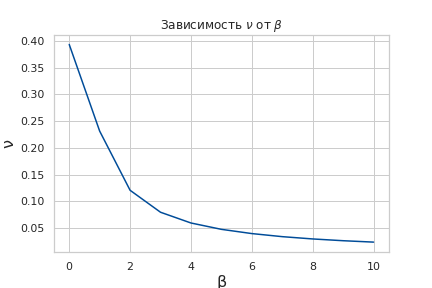
\includegraphics[width=\linewidth]{2ndtaskwithbeta.png}
				\caption{Зависимость обобщенного гауссова числа от $\beta$}
				\label{fig:beta}
			\end{figure*}
		\end{enumerate}
		
	\end{solution}
	\begin{problem}
		Псевдометрическое расстояние между двумя операторами $F(x,y)$ и $G(x,y)$ определяется по формуле:
		\[ d(F,G) = \int_0^1\int_0^1 |F(x,y) - G(x,y)|dxdy \]
		Найдите его величину для следующей пары нечетких операций:
		\begin{equation*}
		\centering
		\begin{aligned}
		F(x,y) = \min\{1, x+y\}
		\end{aligned}
		\quad\quad
		\centering
		\begin{aligned}
		G(x,y) = \min\left\{1, \frac{x+y+2\rho xy}{1 - \rho^2xy} \right\}
		\end{aligned}
		\end{equation*}
		где $ \rho \in [-1,1] $. Исследуйте зависимость псевдометрического расстояния от $\rho$.
	\end{problem}
	\begin{solution}
		Заметим, что $\min\{a,b\} = \frac{a + b - |a-b|}{2}$, а тогда можно записать расстояние между операторами как:
		\[
			d(F,G) = \int_0^1\int_0^1 \abs{\frac{1 + x+y - \abs{x+y-1}}{2} - \frac{1 + \frac{x+y+2\rho xy}{1 - \rho^2xy} - \abs{ 1 - \frac{x+y+2\rho xy}{1 - \rho^2xy}}}{2} }dxdy
		\]
		Используя {\it Python}, исследуем зависимость $d$ от $\rho$, получаем следующий график(рис. \ref{fig:3task}).
		\begin{figure*}[!hbtp]
			\centering
			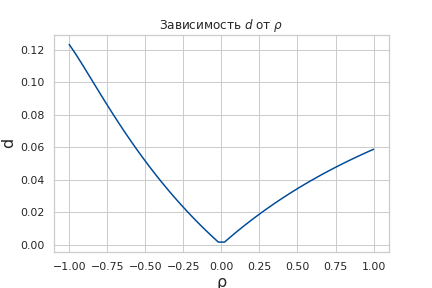
\includegraphics[width=\linewidth]{3task.png}
			\caption{Зависимость $d$ от $\rho$}
			\label{fig:3task}
		\end{figure*}
	\end{solution}
	\newpage
	\begin{problem}
		Непрерывная, строго убывающая функция $ \varphi\colon[0,1] \rightarrow [0, \infty)$, такая что $ \phi(1) = 0$, называется {\bf убывающим} генератором.
		\newline
		Непрерывная строго возрастающая функция $ \varphi\colon[0,1] \rightarrow [0, \infty)$, такая что $ \phi(0) = 0$, называется {\bf возрастающим} генератором.
		\newline
		Найти условия, при которых функция $ \varphi(x) = \frac{1}{2+\alpha}\ln \left( \frac{3-2x}{\alpha(x-1) + 1} \right) + C$ является возрастающим и/или убывающим генератором. Найдите соответствующие треугольные нормы и конормы. Подтвердите графически Ваши выводы.
	\end{problem}
	\begin{solution}
		Сначала найдем условия, при которых $\varphi$ -- возрастающий генератор
		\subparagraph{Условия, при которых $\varphi$ -- возрастающий генератор.}
		Для того, чтобы найти $C$ воспользуемся условием $ \varphi(0) = 0$, тогда:
		\begin{gather*}
			\frac{1}{2+\alpha}\ln \left( \frac{3}{1-\alpha} \right) + C = 0 \Rightarrow \\
			C = \frac{1}{2+\alpha}\ln \left( \frac{1-\alpha}{3} \right)
		\end{gather*}
		Тогда исследуемая функция имеет вид:
		\begin{gather*}
			\xi(x) = \frac{1}{2+\alpha}\ln \left( \frac{3-2x}{\alpha(x-1) + 1} \right) + \frac{1}{2+\alpha}\ln \left( \frac{1-\alpha}{3} \right) = \\
			 \frac{1}{2+\alpha}  \ln\left( \frac{(3-2x)(1-\alpha)}{3(\alpha(x-1) + 1)} \right)
		\end{gather*}
		Функция $\xi$ существует, если $ \frac{(3-2x)(1-\alpha)}{3(\alpha(x-1) + 1)} > 0 $ и $ x \neq 1 - \frac{1}{\alpha} $. Тогда рассмотрим неравенство $ \frac{(3-2x)(1-\alpha)}{3(\alpha(x-1) + 1)} > 0$, равносильное одной из следующих систем:
		\begin{gather*}
			\left\{
				\begin{aligned}
				&(3-2x)(1-\alpha) > 0 \\
				& 3(\alpha(x-1) + 1) > 0
				\end{aligned}
			\right.
			\text{  или  }
			\left\{
			\begin{aligned}
			&(3-2x)(1-\alpha) < 0 \\
			& 3(\alpha(x-1) + 1) < 0
			\end{aligned}
			\right.
		\end{gather*}
		Решая первое неравенство первой системы находим, что $ x > \frac{3}{2}$, а значит первая система не подходит, так как $ x \in [0,1]$. Тогда рассмотрим 2-ую систему:
		\[
			\left\{
			\begin{aligned}
			&(3-2x)(1-\alpha) < 0 \\
			&\alpha(x-1) + 1 < 0
			\end{aligned}
			\right.
		\]
		Решаем систему относительно $\alpha$, помня о том, что $ x \in [0,1]$. Получаем:
		\[
		\left\{
		\begin{aligned}
		&x(2\alpha - 2) < (3 - 3\alpha) \\
		&\alpha x < \alpha-1
		\end{aligned}
		\right.
		\Rightarrow 
		\left\{
		\begin{aligned}
		&x > -\frac{3}{2} \\
		&x < 1 - \frac{1}{\alpha}
		\end{aligned}
		\right.
		\]
		Тогда имеем:
		\begin{enumerate}
			\item $ \alpha \in (-\infty; 0) $, получаем:
			\[
				1 - \frac{1}{\alpha} > 1 \Rightarrow x < 1
			\]
			\item $ \alpha \in (0;1) $, имеем:
			\[
				1 - \frac{1}{\alpha} < 0 \Rightarrow x< 0
			\]
			\item $ \alpha \in (1; \infty) $, получаем:
			\[
				0 <  1 - \frac{1}{\alpha} < 1 \Rightarrow x \in (0,1)
			\]
		\end{enumerate}
		Значит $ \alpha \in (-\infty; 0) \cup (1, \infty) $. Теперь найдем производную:
		\[
			\xi'(x) = \frac{1}{(2x-3)(\alpha(x-1)+1)}
		\]
		Видно, что производная больше $0$, когда $\alpha > 1$, а значит $ \alpha \in (1, \infty) $. Построим возрастающий генератор для различных значений $\alpha$, используя {\it Python}(рис. \ref{fig:incr}).
		\begin{figure*}[!hbtp]
			\centering
			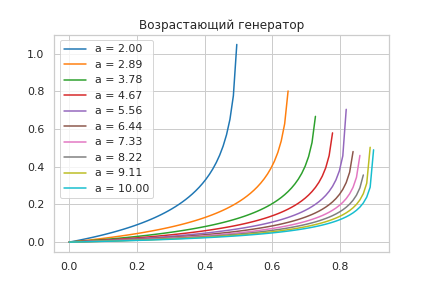
\includegraphics[width=\linewidth]{incr.png}
			\caption{Возрастающий генератор при различных значениях $\alpha$}
			\label{fig:incr}
		\end{figure*}
		\newline
		Теперь найдем коэффициенты функции $ F(x,y) = \frac{a_0 + a_1(x+y) + a_2xy}{b_0 + b_1(x+y) + b_2xy} $, на основе которой можно построить треугольную конорму. Так как генератор имеет вид $ \ln\frac{ax + b}{cx+d} $, то будем искать коэффициенты следующим способом:
		\begin{gather*}
			a_0 = \frac{db^2 - bd^2}{ad-bc},\;a_1 = \frac{bd(a-c)}{ad-bc},\;a_2 = \frac{a^2d-bc^2}{ad-bc} \\
			b_0 = \frac{ad^2 - cb^2}{ad-bc},\;b_1 = \frac{ac(d-b)}{ad-bc},\;b_2 = \frac{ac^2-a^2c}{ad-bc} \\
		\end{gather*}
		Тогда получаем:
		\begin{gather*}
		a_0 = -3,\;a_1 = \frac{3(2+\alpha)}{2},\;a_2 = \frac{9\alpha^2-4(1-\alpha^2)}{2(1-\alpha)} \\
		b_0 = \frac{9\alpha - 6(\alpha-1)}{2},\;b_1 = 0,\;b_2 = \frac{2\alpha(\alpha-1) - 3\alpha^2}{1-\alpha} \\
		\end{gather*}
		Тогда функция имеет вид:
		\[
			F(x,y) = \frac{-3 + \frac{3(2+\alpha)}{2}(x+y) + \frac{9\alpha^2-4(1-\alpha^2)}{2(1-\alpha)}xy}{\frac{9\alpha - 6(\alpha-1)}{2} + \frac{2\alpha(\alpha-1) - 3\alpha^2}{1-\alpha}xy}
		\]
		%
		%Idk how to go forward
		%
		%\iffalse
		$F$ является коммутативной и ассоциативной; определим ограничения на $\alpha$, при выполнении которых $F$ -- Т-конорма.
		\newline
		Проверим, что $F(x,0) = x$:
		\begin{gather*}
			F(x,1) = \frac{-3 + \frac{3(2+\alpha)}{2}(x)}{\frac{9\alpha - 6(\alpha-1)}{2}} = ...
		\end{gather*}
		Вероятно, данная функция не является Т-конормой.
		%\fi
		\subparagraph{Условия, при которых $\varphi$ -- убывающий генератор.}
		Сначала воспользуемся условием, что $ \varphi(1) = 0 $, дабы найти $C$:
		\[
			\frac{1}{2+\alpha}\ln 1 + C = 0
		\]
		Значит $ C = 0$, тогда исследуемая функция имеет вид:
		\[
			\xi(x) = \frac{1}{2+\alpha}\ln \left( \frac{3-2x}{\alpha(x-1) + 1} \right)
		\]
		Функция $\xi$ существует, когда $ \frac{3-2x}{\alpha(x-1) + 1} > 0 $ и $ x \neq 1 - \frac{1}{\alpha} $. Тогда рассмотрим неравенство $ \frac{3-2x}{\alpha(x-1) + 1} > 0 $, равносильное одной из следующих систем:
		 \begin{gather*}
		 \left\{
		 \begin{aligned}
		 &3-2x > 0 \\
		 & \alpha(x-1) + 1 > 0
		 \end{aligned}
		 \right.
		 \text{  или  }
		 \left\{
		 \begin{aligned}
		 &3-2x < 0 \\
		 & \alpha(x-1) + 1 < 0
		 \end{aligned}
		 \right.
		 \end{gather*}
		 Решая первое неравенство второй системы находим, что $ x > \frac{3}{2}$, а значит вторая система не подходит, так как $ x \in [0,1]$. Тогда рассмотрим 1-ую систему:
		 \[
		 \left\{
		 \begin{aligned}
		 &3-2x > 0 \\
		 & \alpha(x-1) + 1 > 0
		 \end{aligned}
		 \right.
		 \Rightarrow 
		 \left\{
		 \begin{aligned}
		 &x < \frac{3}{2} \\
		 &x > \frac{1}{\alpha} - 1
		 \end{aligned}
		 \right.
		 \]
		 Тогда имеем:
		 \begin{enumerate}
		 	\item $ \alpha \in (-\infty; 0) $, получаем:
		 	\[
		 	 \frac{1}{\alpha} - 1 < 0 \Rightarrow x > 0
		 	\]
		 	\item $ \alpha \in (0;1) $, имеем:
		 	\[
		 	\frac{1}{\alpha} - 1 \geq 1 \Rightarrow x> 1
		 	\]
		 	\item $ \alpha \in [1; \infty) $, получаем:
		 	\[
		 	 \frac{1}{\alpha} - 1 \leq 0 \Rightarrow x \geq 0
		 	\]
		 \end{enumerate}
		 Значит $ \alpha \in (-\infty; 0) \cup [1, \infty) $.Теперь найдем производную:
		 \[
		 \xi'(x) = \frac{1}{(2x-3)(\alpha(x-1)+1)}
		 \]
		 Видно, что производная меньше $0$, когда $\alpha < 1$, а значит $ \alpha \in (-\infty; 0) \setminus \{ -2 \} $. Построим убывающий генератор для различных значений $\alpha$, используя {\it Python}(рис. \ref{fig:decr}).
		 \begin{figure*}[!hbtp]
		 	\centering
		 	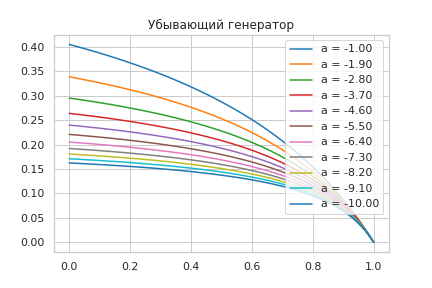
\includegraphics[width=\linewidth]{decr.png}
		 	\caption{Возрастающий генератор при различных значениях $\alpha$}
		 	\label{fig:decr}
		 \end{figure*}
	 \newline
	 Теперь найдем коэффициенты функции $ F(x,y) = \frac{a_0 + a_1(x+y) + a_2xy}{b_0 + b_1(x+y) + b_2xy} $, на основе которой можно построить треугольную норму. Коэффициенты имеют вид:
	 \begin{gather*}
	 a_0 = 3(\alpha-1),\;a_1 = 3(1-\alpha),\;a_2 = \frac{3\alpha^2 + 4\alpha - 4}{2+\alpha} \\
	 b_0 = \frac{2+7\alpha}{2+\alpha},\;b_1 = -2\alpha,\;b_2 = 2 \\
	 \end{gather*}
	 Тогда функция $F$ имеет вид:
	 \[
	 	F(x,y) = \frac{3(\alpha-1) + 3(1-\alpha)(x+y) + \frac{3\alpha^2 + 4\alpha - 4}{2+\alpha}xy}{\frac{2+7\alpha}{2+\alpha} + -2\alpha(x+y) + 2xy}
	 \]
	 $F$ является коммутативной и ассоциативной; определим ограничения на $\alpha$, при выполнении которых $F$ -- Т-норма.
	 \newline
	 Проверим, что $F(x,1) = x$:
	 \begin{gather*}
	 F(x,1) = \frac{3(\alpha-1) + 3(1-\alpha)(x+1) + \frac{3\alpha^2 + 4\alpha - 4}{2+\alpha}x}{\frac{2+7\alpha}{2+\alpha} + -2\alpha(x+1) + 2x} = \\
	 \frac{3(1-\alpha)(2+\alpha)x + (3\alpha^2 + 4\alpha-4)x}{ 2 + 3\alpha +4x - 2\alpha x-2\alpha -2\alpha^2x } = ...
	 \end{gather*}
	 Вероятно, данная функция не является Т-нормой.
	\end{solution}
\end{document}